\documentclass[journal,lettersize]{IEEEtran}

\usepackage[utf8]{inputenc}
\usepackage[T1]{fontenc}
\usepackage{graphicx}
\usepackage{hyperref}

\hypersetup{colorlinks=true,linkcolor=blue,citecolor=blue,urlcolor=blue}

\begin{document}

\title{Supplementary Material for: Global Fundamental-Parameter Mapping of Lunar Elemental Abundances from Chandrayaan-2 CLASS XRF Data with Cross-Modal Super-Resolution}

\author{Smarak~Kanjilal, Subarno~Maji, \emph{and} Paidi~Geetesh~Chandra}

\maketitle
\renewcommand{\thefigure}{S\arabic{figure}}

\section*{Overview}

This document provides supplementary figures for the manuscript
``Global Fundamental-Parameter Mapping of Lunar Elemental Abundances
from Chandrayaan-2 CLASS XRF Data with Cross-Modal Super-Resolution.''
The main text restricts the cross-modal guided super-resolution
demonstration to aluminium (Fig.~3 of the main paper), the element with
both the strongest optical--compositional correlation and the
best-validated ground-truth agreement. Table~II of the main paper
already reports the Pearson correlation coefficients between optical
intensity and element/Si abundance ratio for all six mapped elements
(Al, Mg, O, Fe, Ca, Ti), which is the quantitative basis for that
choice; the figures below show the corresponding before/after
super-resolution maps for the four next most relevant elements
(Mg, Ca, Fe, Ti) for readers who wish to inspect them directly, together
with a supplementary view of the global spatial coverage underlying the
99.0\% coverage claim in Section~VII-B of the main paper. As in the main
paper, all concentrations are relative scale factors, not calibrated
weight percent (see Section~IV-A of the main paper), and the
super-resolution maps are restricted to the $|\phi|<60^{\circ}$
reliable band.

\section*{Supplementary Figures}

\begin{figure*}[!t]
  \centering
  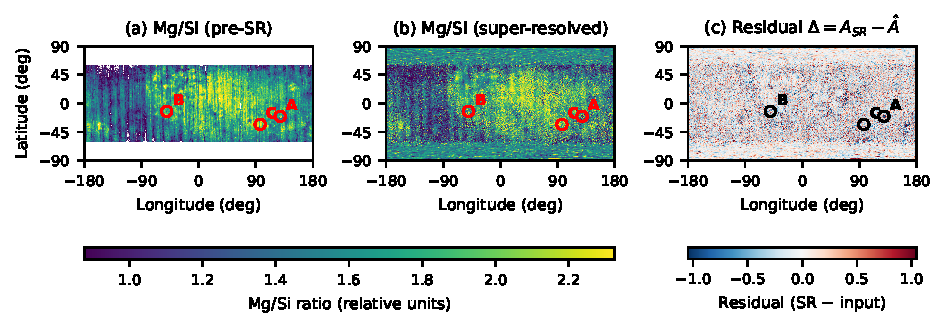
\includegraphics[width=\textwidth]{../outputs/figures/supplementary/supp_sr_Mg.pdf}
  \caption{Mg/Si ratio map before (a) and after (b) cross-modal guided
    super-resolution ($\alpha=1.0$, full detail injection, see main-paper
    Table~IV for the blending-weight ablation), shown on the
    $|\phi|<60^{\circ}$ analysis band, plus (c) the explicit residual
    $\Delta = \mathbf{A}_{\mathrm{SR}} - \hat{\mathbf{A}}$ (diverging
    colour scale, white = no change). Mg has a strong optical correlation
    ($\rho=-0.39$, main-paper Table~II) but is not confirmed by
    ground-truth validation ($r=+0.006$, main-paper Table~V, effectively
    null). Colorbar units in (a)/(b) are the relative Mg/Si ratio, not
    wt\%.}
  \label{fig:supp_mg}
\end{figure*}

\begin{figure*}[!t]
  \centering
  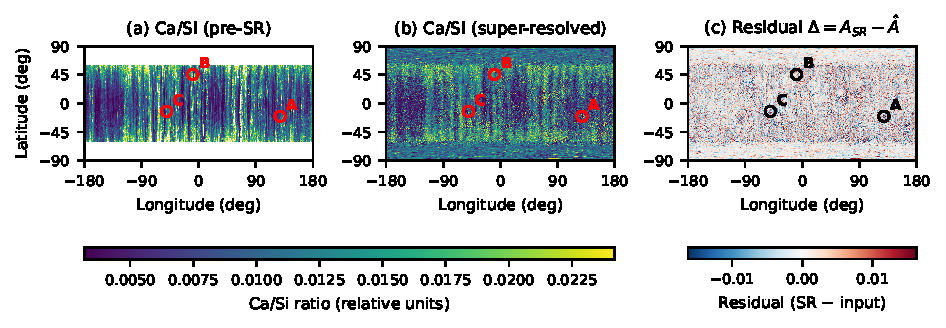
\includegraphics[width=\textwidth]{../outputs/figures/supplementary/supp_sr_Ca.pdf}
  \caption{Ca/Si ratio map before (a) and after (b) cross-modal guided
    super-resolution ($\alpha=1.0$, full detail injection), shown on the
    $|\phi|<60^{\circ}$ analysis band, plus (c) the explicit residual
    $\Delta = \mathbf{A}_{\mathrm{SR}} - \hat{\mathbf{A}}$. Ca has a weak
    optical correlation ($\rho=+0.02$, main-paper Table~II) but the
    best ground-truth validation after Al ($r=+0.263$, main-paper
    Table~V). Colorbar units in (a)/(b) are the relative Ca/Si ratio,
    not wt\%.}
  \label{fig:supp_ca}
\end{figure*}

\begin{figure*}[!t]
  \centering
  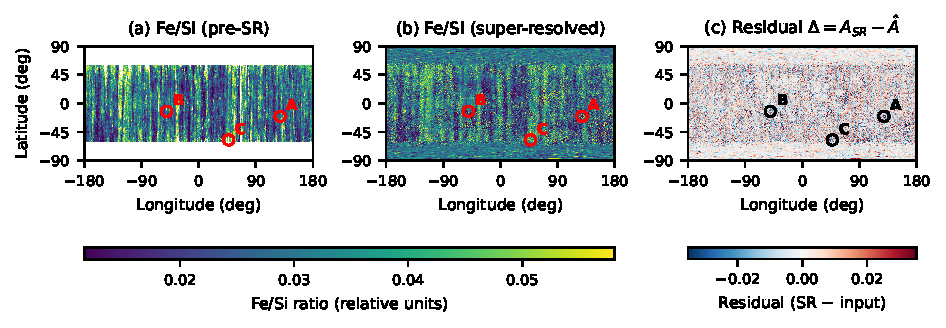
\includegraphics[width=\textwidth]{../outputs/figures/supplementary/supp_sr_Fe.pdf}
  \caption{Fe/Si ratio map before (a) and after (b) cross-modal guided
    super-resolution ($\alpha=1.0$, full detail injection), shown on the
    $|\phi|<60^{\circ}$ analysis band, plus (c) the explicit residual
    $\Delta = \mathbf{A}_{\mathrm{SR}} - \hat{\mathbf{A}}$. Fe has a weak
    optical correlation ($\rho=+0.10$, main-paper Table~II) and
    essentially no ratio-space ground-truth correlation
    ($r=-0.002$, main-paper Table~V), so this map carries little
    evidential support on either axis and should not be interpreted with
    the confidence of the Al headline result. Colorbar units in (a)/(b)
    are the relative Fe/Si ratio, not wt\%.}
  \label{fig:supp_fe}
\end{figure*}

\begin{figure*}[!t]
  \centering
  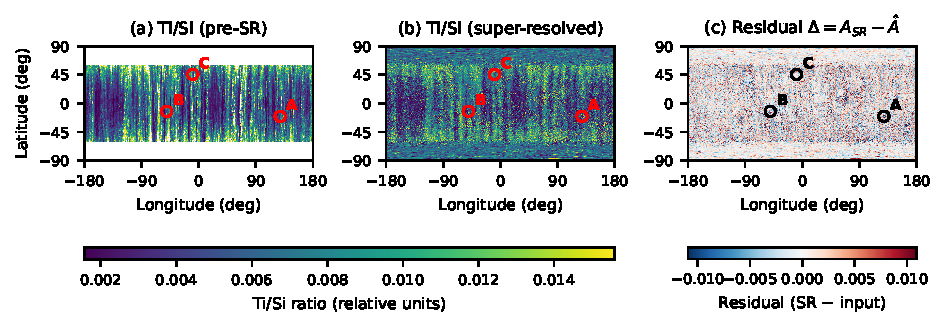
\includegraphics[width=\textwidth]{../outputs/figures/supplementary/supp_sr_Ti.pdf}
  \caption{Ti/Si ratio map before (a) and after (b) cross-modal guided
    super-resolution ($\alpha=1.0$, full detail injection), shown on the
    $|\phi|<60^{\circ}$ analysis band, plus (c) the explicit residual
    $\Delta = \mathbf{A}_{\mathrm{SR}} - \hat{\mathbf{A}}$. Ti has a
    negligible optical correlation ($\rho=+0.01$, main-paper Table~II)
    and a weak negative ground-truth correlation ($r=-0.117$, main-paper
    Table~V), so this map carries little evidential support on either
    axis and should not be interpreted with the confidence of the Al
    headline result. Colorbar units in (a)/(b) are the relative Ti/Si
    ratio, not wt\%.}
  \label{fig:supp_ti}
\end{figure*}

\begin{figure}[!t]
  \centering
  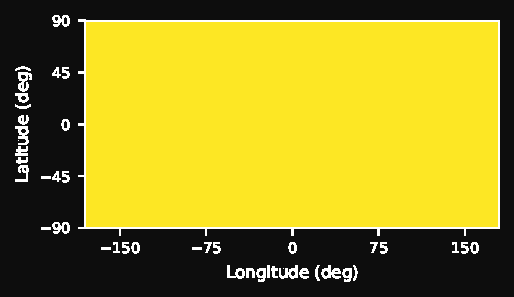
\includegraphics[width=\linewidth]{../outputs/figures/supplementary/supp_coverage.pdf}
  \caption{Per-cell footprint density (log-scaled count of dayside
    spectra landing in each $1^{\circ}\times1^{\circ}$ cell) underlying
    the 99.0\% global coverage figure reported in Section~VII-B of the
    main paper; the coverage statistic itself is the binary
    occupied/unoccupied threshold of this same count array. Vertical
    banding traces repeated ground-track passes, with density rising
    toward the poles where tracks converge; the darkest streaks are the
    540/64{,}800 cells ($0.83\%$) with zero footprints, which are what
    the near-uniform 99.0\% coverage figure represents.}
  \label{fig:supp_coverage}
\end{figure}

\end{document}
